\documentclass[openany,12pt,a4paper]{report}
\usepackage{subfiles}
\usepackage[]{graphicx}
\usepackage{float}
\usepackage{multirow}
\graphicspath{{./img/}{./../img/}}
\usepackage{../StileDoc}
\title{Product Baseline - Allegato tecnico}
\author{}

\loadglsentries{../Glossario/Definizioni}
%Ultima versione documento

\newcommand{\versione}{}

\begin{document}
	\makeatletter
	\begin{titlepage}
		\setlength{\headsep}{0pt}  
		\begin{center}
			
\includegraphics[width=0.5\linewidth]{img/Logo.png}\\[1em]
			{\huge \bfseries  \@title }\\[10ex]
			\textbf{\Large Informazioni Documento} \\[2em]
			\bgroup
			\def\arraystretch{1.5}
			\begin{tabular}{l|l}
				\textbf{Distribuzione} & Prof. Tullio Vardanega \\
				& Prof. Riccardo Cardin \\
				& Gruppo Graphite \\
				\textbf{Uso} & Esterno \\
				\textbf{Recapito} & graphite.swe@gmail.com \\
			\end{tabular}
			\egroup
		\end{center}
	\end{titlepage}
	\makeatother
	
	\thispagestyle{empty}
	\newpage
	
	\tableofcontents
	
	\chapter{Introduzione}
	
	\section{Scopo del documento}
	
	Il documento ha la finalità di illustrare la \textit{Product Baseline} (PB in breve) per l’applicazione
	\textit{"DeSpeect: un'interfaccia grafica per Speect"}, con particolare attenzione per lo stato attuale del prodotto, la sua architettura e la copertura di use case e requisiti funzionali obbligatori.
	
	\section{Scopo del prodotto}
	
	Lo scopo del progetto è la realizzazione di un’interfaccia grafica per Speect [Meraka Institute(2008-2013)], una libreria per la creazione di sistemi di sintesi vocale, che agevoli l’ispezione del suo stato interno durante il funzionamento e la scrittura di test per le sue funzionalità.

	\section{Riferimenti}
	
	\subsection*{Riferimenti normativi}
	
	\begin{itemize}
		\item \textbf{Norme di Progetto v3.0.0}: documento \textit{Norme di progetto v3.0.0};
		\subitem §2.2.5 "Progettazione";
		\subitem §4.7.3 "Strumenti relativi allo sviluppo".
	\end{itemize}
	
	\subsection*{Riferimenti informativi}
	
	\begin{itemize}
		\item \textbf{Analisi dei Requisiti v3.0.0}: documento \textit{Analisi dei Requisiti v3.0.0};
		\subitem Definisce nel dettaglio use case e requisiti.
		
		\item \textbf{Documentazione Speect:} \\
		\url{http://speect.sourceforge.net/contents.html};
		\subitem Documentazione ufficiale della libreria di \textit{Text-To-Speech} di riferimento per il progetto.
		
		\item \textbf{Documentazione Qt:} \\
		\url{http://doc.qt.io/};
		\subitem Documentazione ufficiale del framework utilizzato per lo sviluppo dell'interfaccia grafica.
		
		\item \textbf{Documentazione CMAKE:} \\
		\url{https://cmake.org/documentation/}.
		\subitem Documentazione ufficiale del framework utilizzato per la build del prodotto. 
	\end{itemize}

	\chapter{Requisiti di sistema}
	
	L'installazione ed esecuzione del software richiede i seguenti prerequisiti:
	
	\begin{itemize}
		\item Sistema operativo Unix / Unix-like (il software è stato testato solo per piattaforma Ubuntu 16.04 LTS)
		\subitem \url{https://www.ubuntu.com/download/desktop}
		\item CMake (versione minima 2.8)
		\subitem \url{https://cmake.org/download/}
		\item Compilatore ANSI C/ISO C90 GCC (versione minima 5.0)
		\subitem \url{https://gcc.gnu.org/install/binaries.html}
		\item Qt 5.9.0 LTS
		\subitem \url{https://www.qt.io/download}
	\end{itemize}

	\chapter{Installazione ed esecuzione}
	
	Il codice relativo alla Product Baseline è reperibile in un apposito repository GitHub al seguente link:
	\begin{center}
		\url{https://github.com/graphiteSWE/Despeect-ProductBaseline}
	\end{center} 

	\noindent Per installare ed eseguire il software è necessario attenersi alla seguente procedura:
	\begin{enumerate}
		\item Clonare o scaricare la repository sulla propria macchina;
		\item Entrare nella cartella scaricata ed eseguire lo script \verb|build.sh|;
		\item Eseguire da terminale il comando \verb|cd DeSpeect/build/|;
		\item Avviare l'eseguibile con il comando \verb|./main|.
	\end{enumerate}
	Tale procedura installerà la libreria Speect e genererà una build del software nella directory \verb|DeSpeect/build/|, nonché avvierà automaticamente un'esecuzione dello stesso. Ulteriori informazioni, nonché un esempio di procedura di stampa di un grafo, sono reperibili nel file \verb|README.md| del repository.

	\chapter{Rapporto con il PoC}
	Precedentemente alla Product Baseline, è stato realizzato un \textit{Proof of Concept} (PoC in breve) a dimostrazione della fattibilità del prodotto DeSpeect. Tale PoC, che ha rappresentato il punto di partenza per la realizzazione della PB, è tuttora reperibile al seguente link:
	\begin{center}
		\url{https://github.com/graphiteSWE/TB-PoC}
	\end{center}

	\noindent Segue una tabella che evidenzia le differenze tra le caratteristiche del PoC, contestualizzato nel suo scopo, e quelle della PB. \\
	
	\begin{longtable}{|p{70mm}|p{70mm}|}
		\caption {Tabella di confronto tra PoC e PB} \label{tab:Tabella di confronto tra PoC e PB} \\
		\hline
		\textbf{Proof of Concept} & \textbf{Product Baseline} \\
		
		\hline Architettura abbozzata e sommaria, priva di design pattern 
		&
		Architettura basata su MVVM e facente uso di vari design pattern \\ 
		
		\hline Implementazione di un'interfaccia grafica provvisoria e carente di elementi fondamentali per il soddisfacimento di molti requisiti obbligatori 
		&
		Interfaccia grafica quasi completa predisposta all'implementazione della totalità dei requisiti obbligatori \\ 
		
		\hline Implementazione di poche funzionalità dimostrative (per esempio la stampa parziale del grafo)
		&
		Implementazione della maggior parte delle funzionalità richieste dai requisiti funzionali obbligatori \\ 
		
		\hline Modalità di installazione e configurazione macchinose
		&
		Modalità di installazione e configurazione semplificate \\ 
		\hline
	\end{longtable}

	\chapter{Architettura generale del prodotto}
	
	L'architettura generale del prodotto segue il pattern Model-View-ViewModel. Questo pattern è basato su tre componenti principali:
	
	\begin{itemize}
		\item \textbf{Model}: un'implementazione del modello del dominio dei dati;
		\item \textbf{View}: la struttura, il layout e l'aspetto di ciò che l'utente visualizza a schermo;
		\item \textbf{ViewModel}: un'astrazione della view che espone proprietà pubbliche e comandi.
	\end{itemize}
	
	\noindent Esso permette tra le altre cose un totale disaccoppiamento tra logica di business e presentazione, informazioni più dettagliate a riguardo sono reperibili nell'appendice §A "Model-View-ViewModel" di questo documento. I seguenti diagrammi illustrano sinteticamente la struttura del software attraverso i package che lo costituiscono, con livello di dettaglio crescente.
	
	\newpage
	
	\begin{figure}[H]
		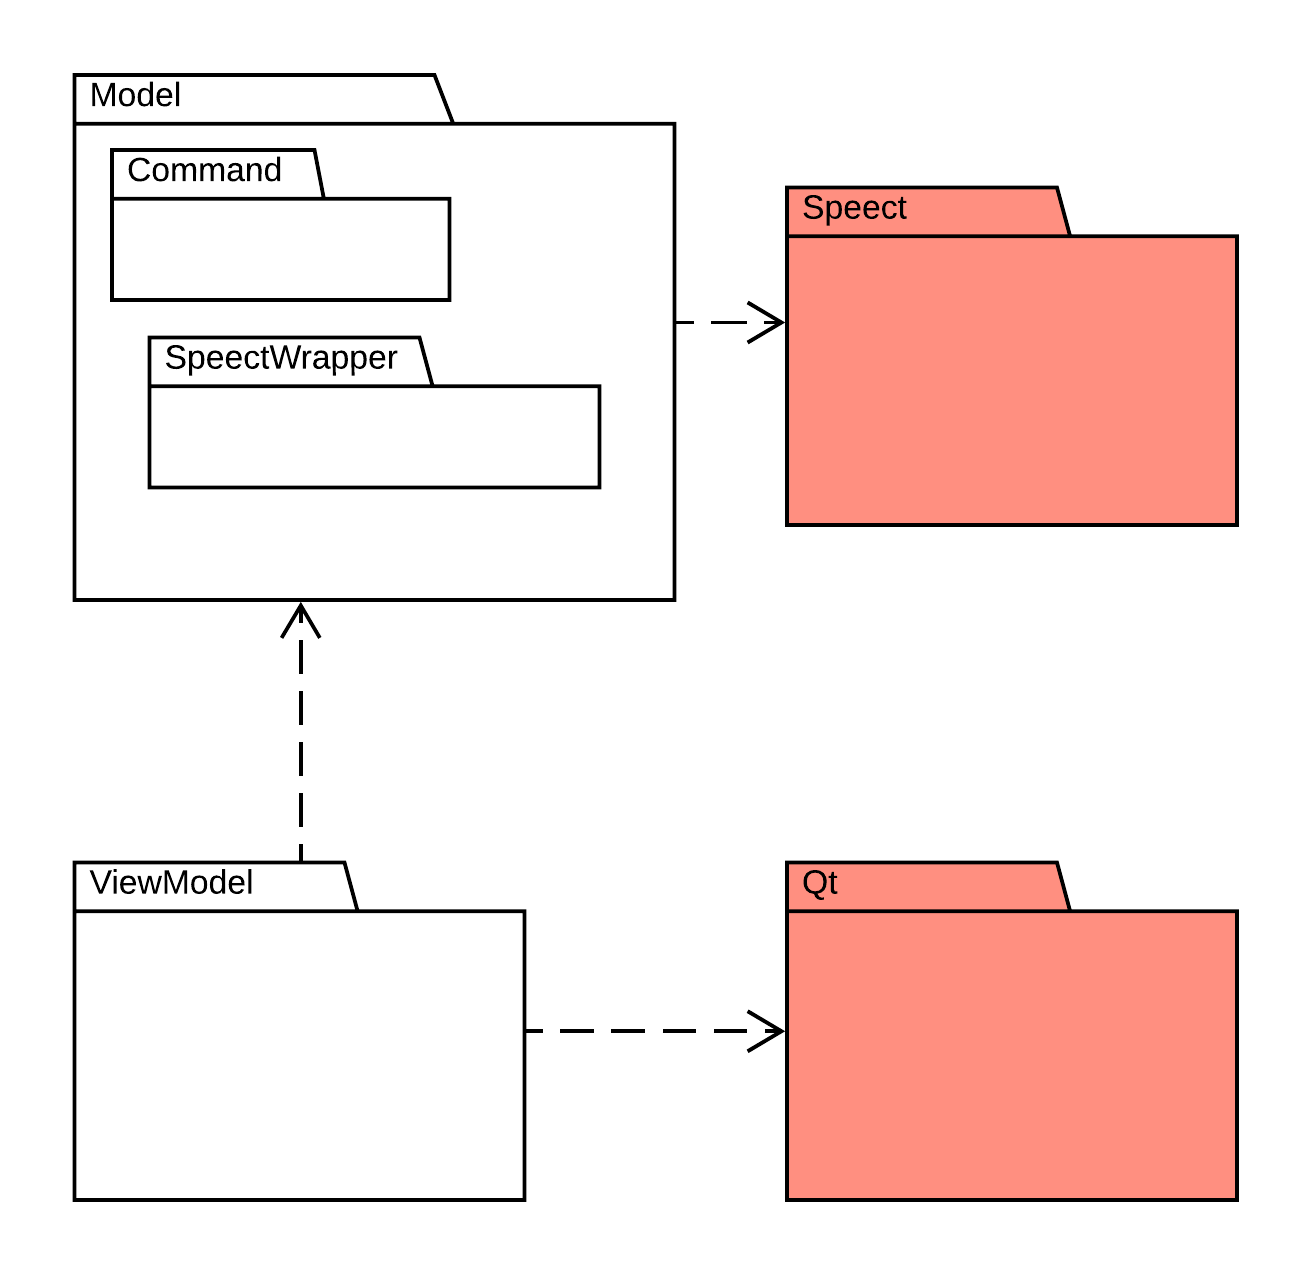
\includegraphics[scale=1.4]{PackageDiagram1}
		\centering
		\caption{Diagramma generale dei package}
	\end{figure}
	
	\newpage
	
	\begin{figure}[H]
		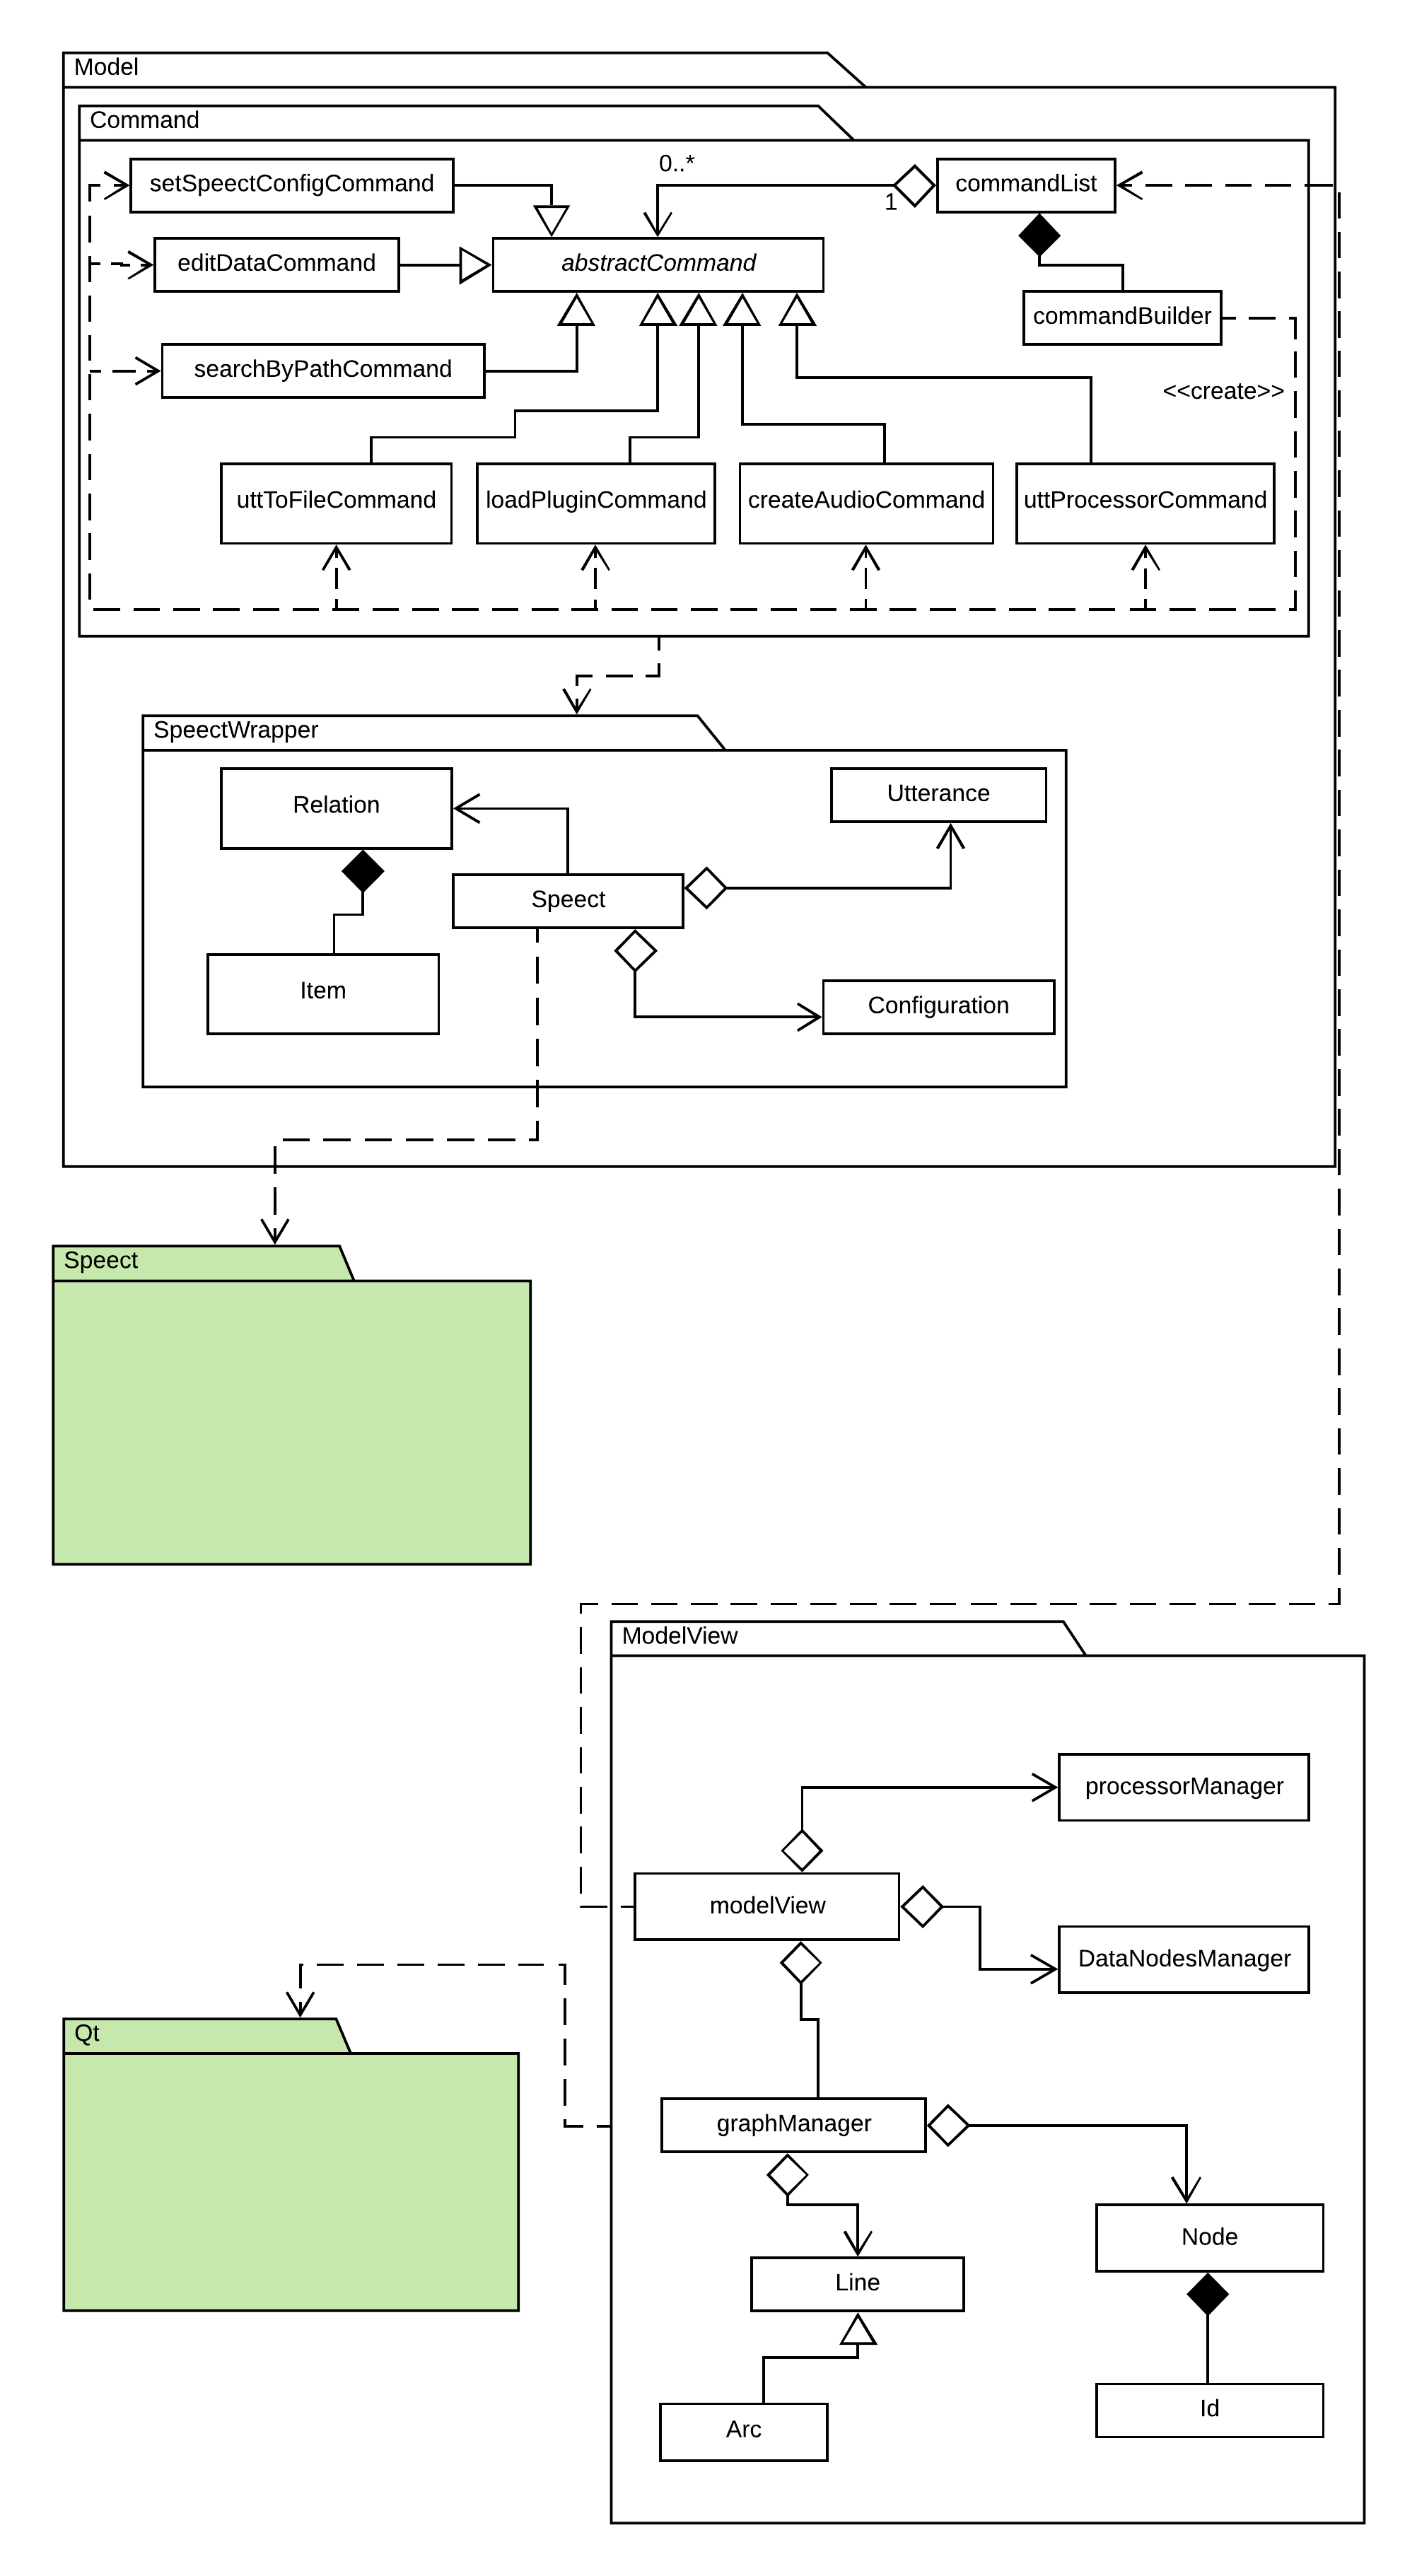
\includegraphics[scale=0.63]{PackageDiagram2}
		\centering
		\caption{Diagramma dei package nel dettaglio}
	\end{figure}
	
	\chapter{Implementazione MVVM}
	
	Vengono di seguito illustrate le implementazioni per le componenti del pattern Model-View-ViewModel in relazione all'architettura della Product Baseline. Per ogni componente, vengono illustrati:
	
	\begin{itemize}
		\item \textbf{Contestualizzazione}: spiegazione generale dell'architettura del componente all'interno del sistema.
		\item \textbf{Diagramma delle classi}: diagramma generale delle classi per il componente. Per motivi di spazio e leggibilità, il diagramma qui riportato è una versione semplificata priva dell'indicazione di tutti i metodi. I diagrammi completi sono disponibili sul repository dedicato alla PB nell'apposita directory \verb|Diagrammi/DiagrammiClassi/|;
		\item \textbf{Design Pattern}: una descrizione e contestualizzazione esaustiva dei design pattern impiegati all'interno del componente.
	\end{itemize} 
	
	\section{View}
	
	La View, conseguentemente all’uso del framework Qt, consiste di un file \textit{qml} trasformato durante la compilazione in classi compatibili C++. Il comportamento della View è indi gestito dal package ViewModel. 
	
	\section{Model}
	
	\subsection{Contestualizzazione}
	
	Nella progettazione del Model è emersa la necessità di interagire con la libreria Speect incapsulandone alcune funzionalità rilevanti. Per realizzare ciò il Model è stato diviso in due package corrispondenti all'implementazione dei design pattern Façade (SpeectWrapper), per quanto riguarda l'incapsulamento della libreria, e Command, per quanto riguarda la suddivisione delle funzionalità implementate in un'ottica di componibilità ed estendibilità.  
	
	\subsection{Diagramma delle classi}
	
	\begin{figure}[H]
		\hspace*{-20mm}
		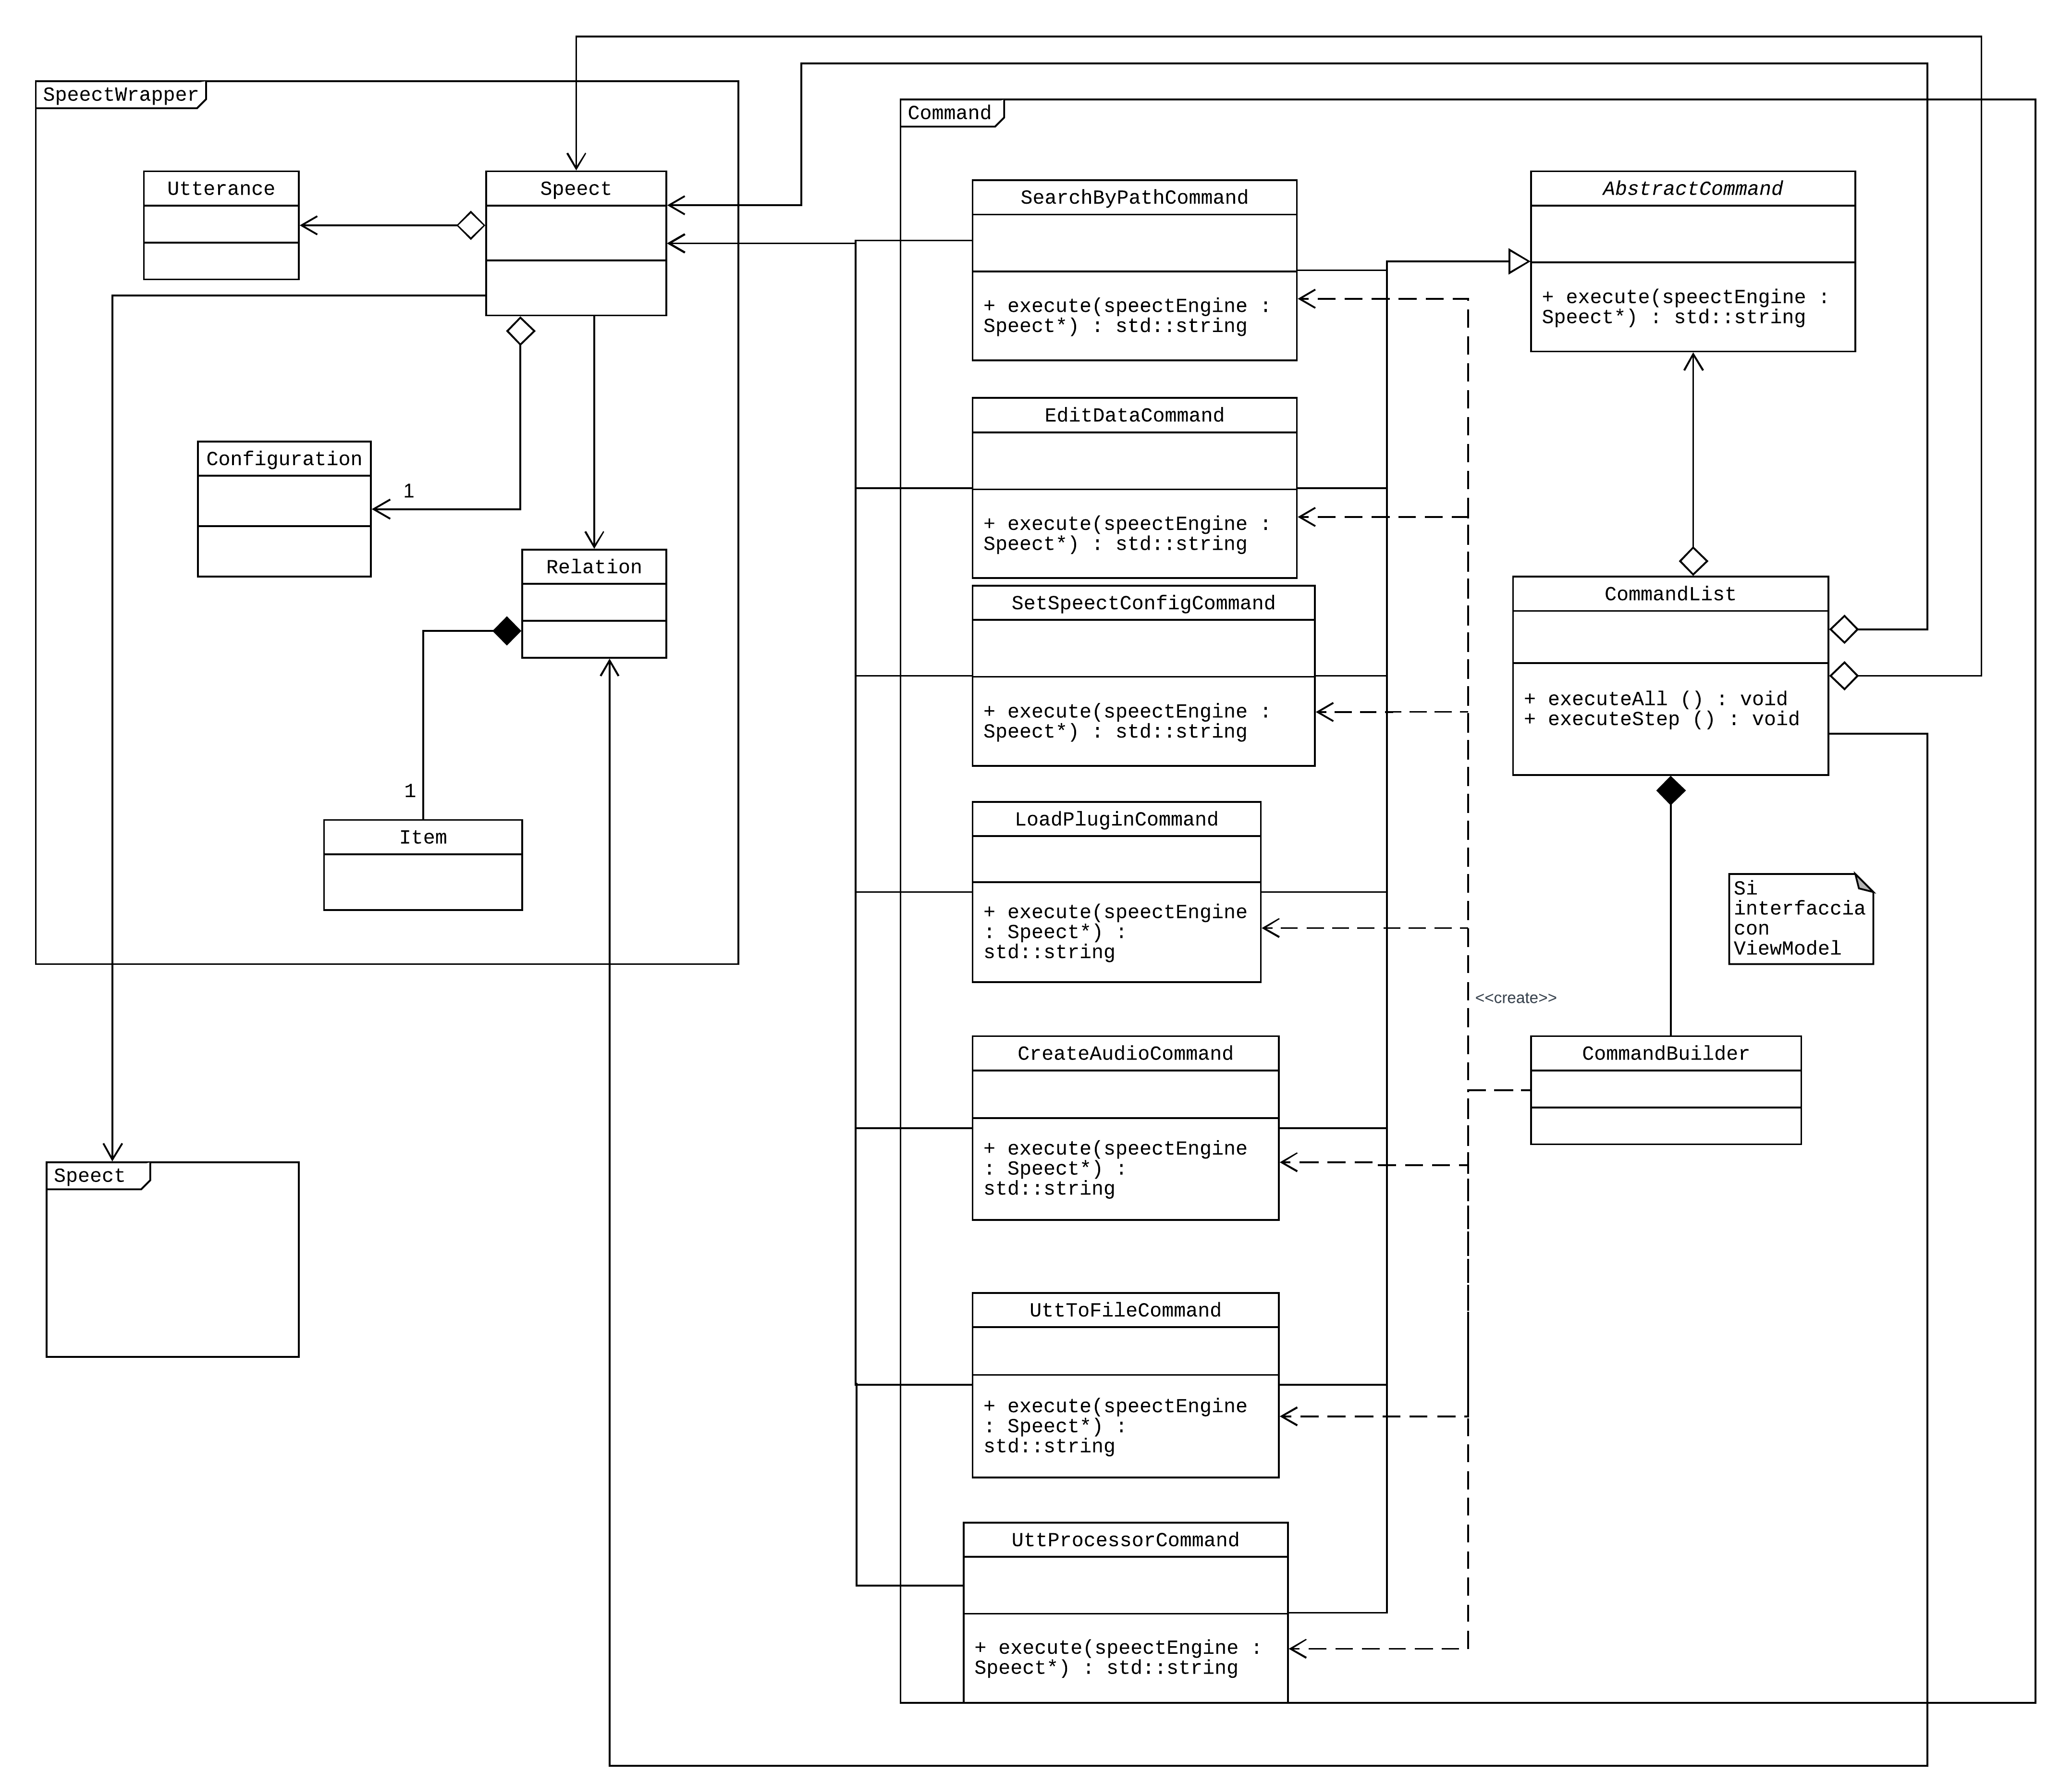
\includegraphics[scale=0.5]{ModelDiagram}
		\centering
		\caption{Diagramma delle classi del componente Model}
	\end{figure}
		
	\newpage
		
	\subsection{Design pattern}
	
	\subsubsection{Command}
	Permette la suddivisione delle funzionalità implementate in un'ottica di componibilità ed estendibilità. I comandi concreti sono aggregati in una lista (\verb|CommandList|) che si interfaccia con la componente ViewModel. Tali comandi interagiscono a loro volta con il package SpeectWrapper per ottere i dati da elaborare dalla libreria Speect. Ai comandi è delegata l'esecuzione degli utterance processor per la successiva stampa dei dati nel grafo, ma anche l'implementazione di funzionalità quali il caricamento dei plug-in e della configurazione di Speect.
	
	\subsubsection{Builder}
	Questo design pattern separa la costruzione di un oggetto complesso dalla sua rappresentazione, cosicché il processo di costruzione stesso possa creare diverse rappresentazioni. Contestualizzato nel sistema della PB, esso si interfaccia con il ViewModel per la configurazione e costruzione di una specifica \verb|CommandList|.
	
	\subsubsection{Façade} 
	Il design pattern Façade permette, attraverso un'interfaccia più semplice, l'accesso a sottosistemi che espongono interfacce complesse e molto diverse tra loro, nonché a blocchi di codice complessi. In questo contesto, il package SpeectWrapper incapsula la libreria Speect rendendola accessibile tramite omonima classe proprietaria.
	
	\newpage
	
	\section{ViewModel}
	
	\subsection{Contestualizzazione}
	Il package ViewModel funge da tramite tra Model e View, prelevando i dati dal primo per aggiornare il secondo. Per quanto riguarda la stampa del grafo, la classe \verb|GraphManager| si occupa di aggiornarne la presentazione interfacciandosi con le librerie Qt e con le classi \verb|Line|, \verb|Arc| e \verb|Node|.  
	
	\subsection{Diagramma delle classi}
		
	\begin{figure}[H]
		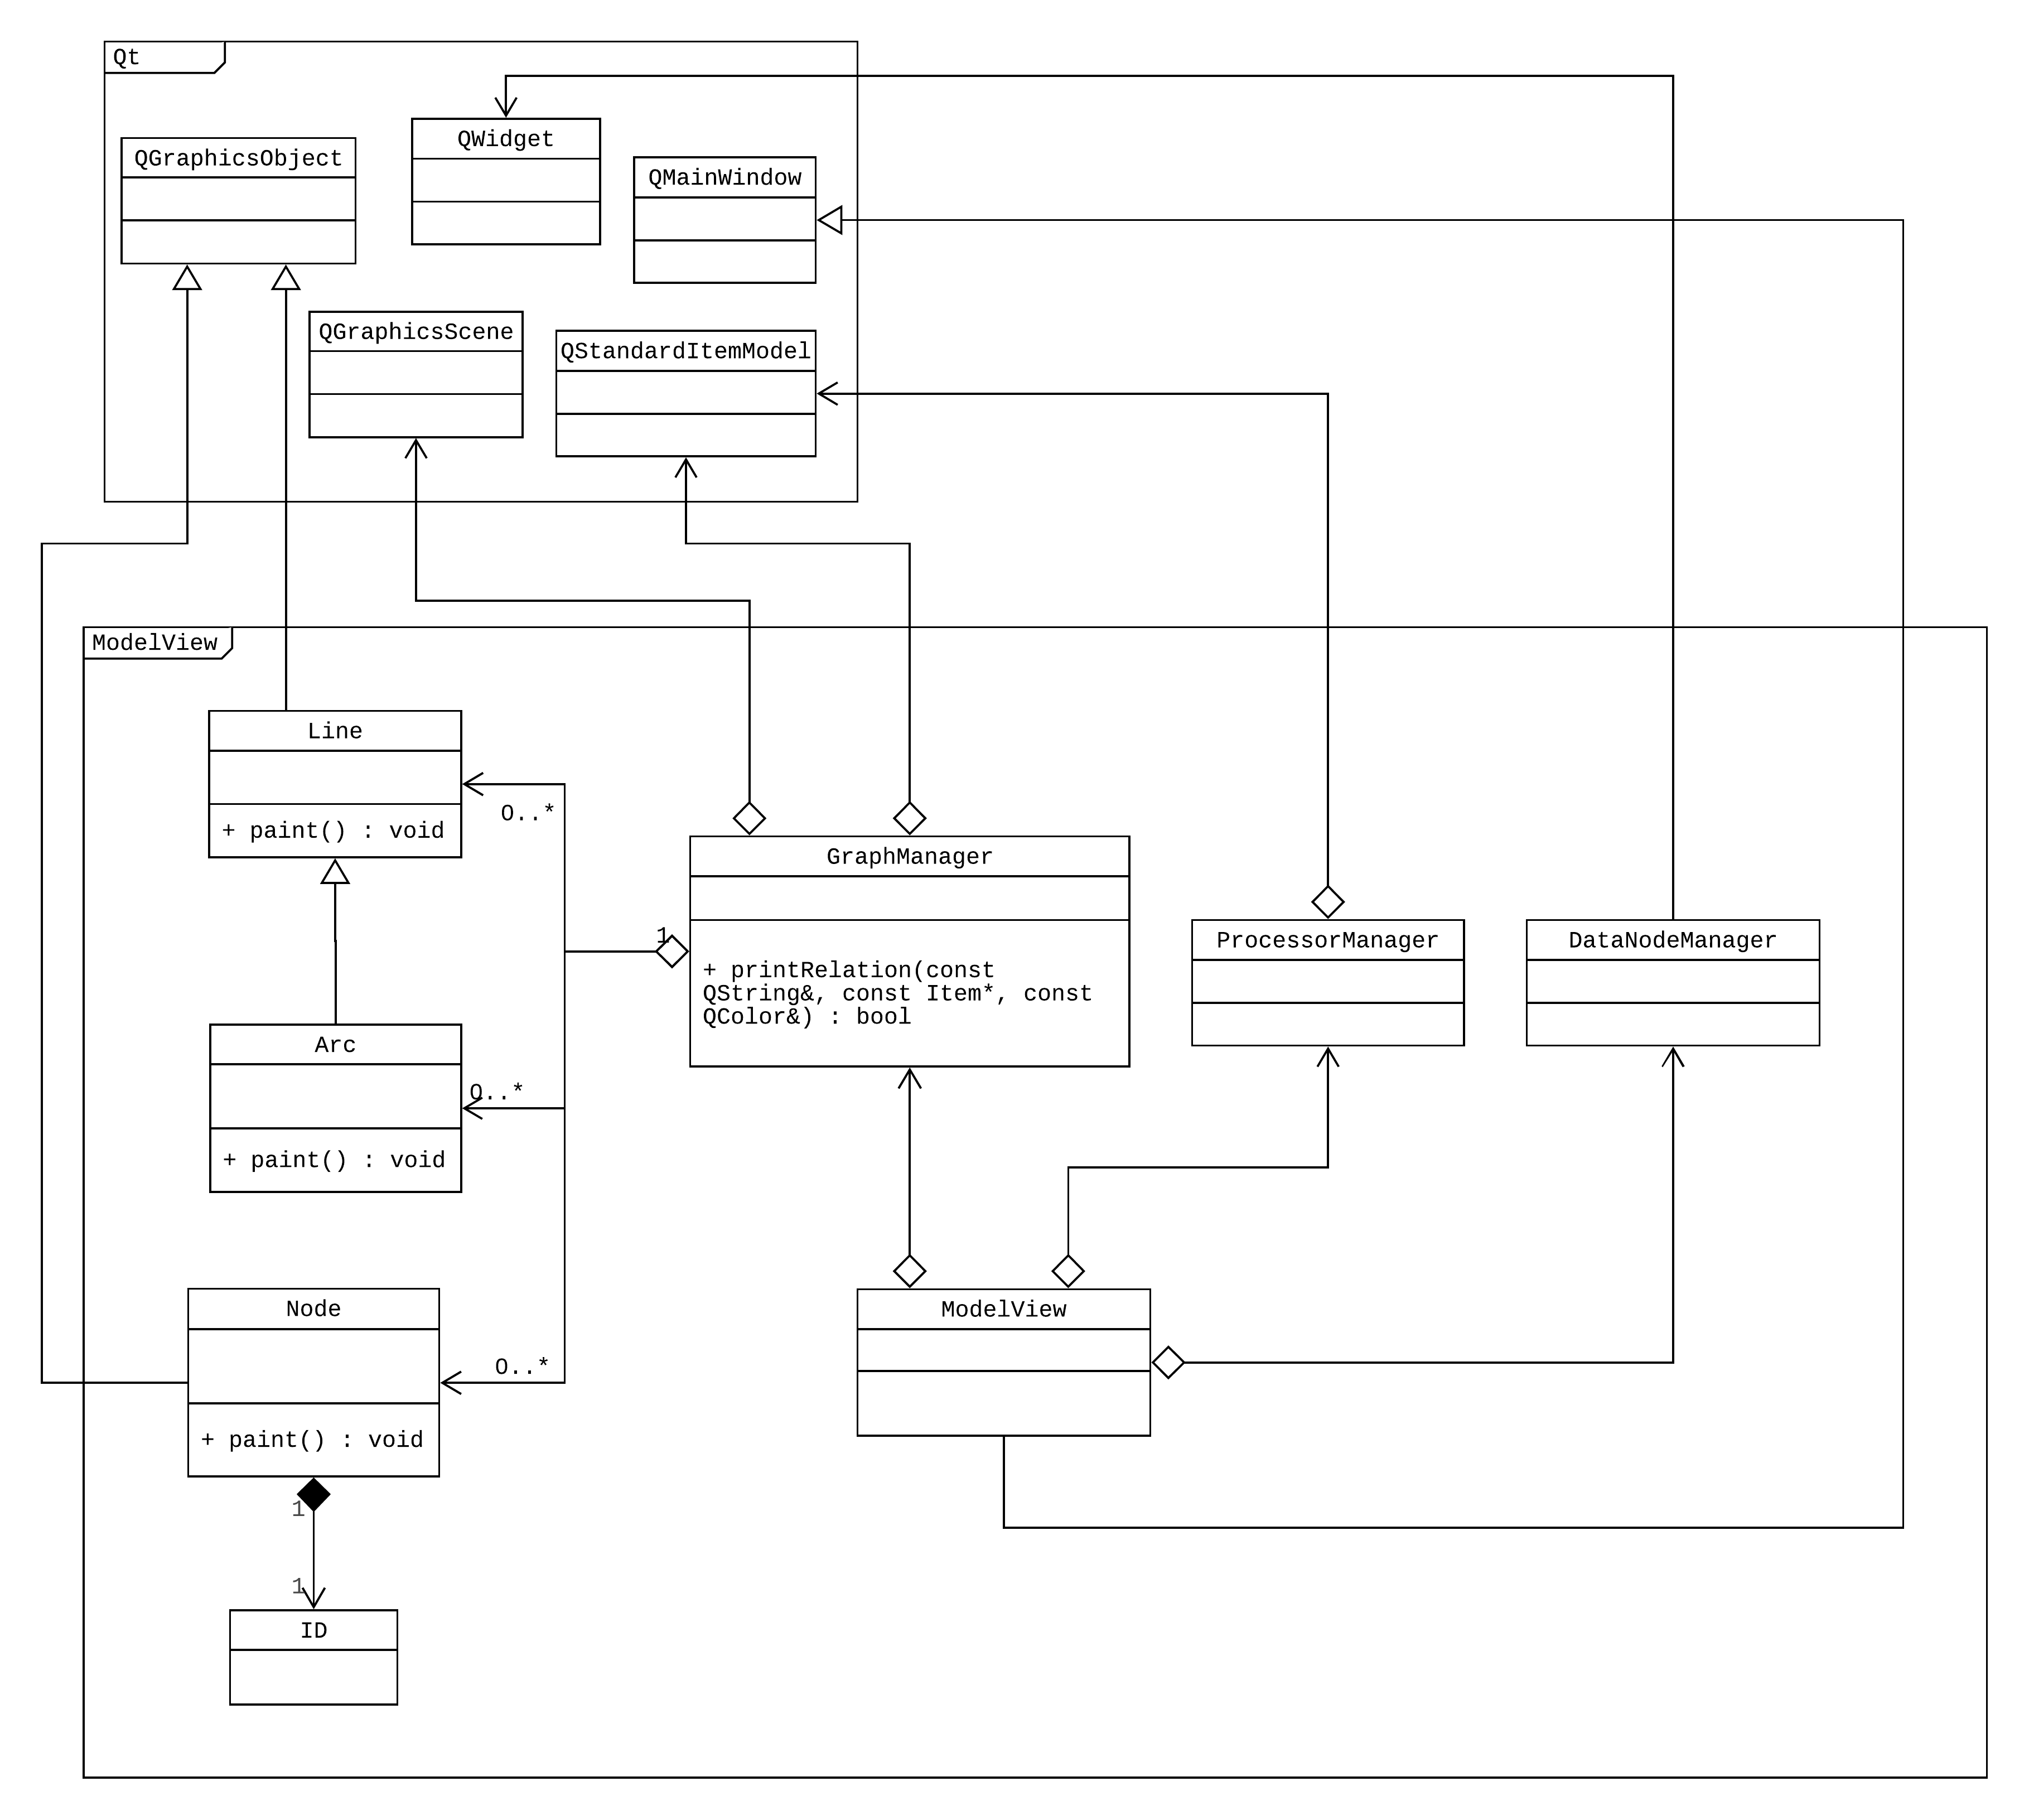
\includegraphics[scale=0.5]{ViewModelDiagram}
		\centering
		\caption{Diagramma delle classi del componente ViewModel}
	\end{figure}

	\subsection{Design pattern}
	
	\subsubsection{Observer}
	Il framework Qt, attraverso il sistema di signal e slot, implementa tale design pattern. Esso permette di reagire efficientemente ad un cambiamento dell'interfaccia grafica, chiedendo se necessario l'aggiornamento dei dati del Model attraverso il ViewModel. Il meccanismo di signal e slot è implementato dalle classi pertinenti all'interno del package.  

	\newpage

	\section{Diagrammi di sequenza}
	
	Vengono qui presentati i diagrammi di sequenza per alcune richieste notevoli. Si noti che tali diagrammi sono disponibili all'interno del repository nella directory \verb|Diagrammi/DiagrammiSequenza/|.
	
	\subsection{Caricamento voice}
	
	Il seguente diagramma di sequenza rappresenta il processo di caricamento e configurazione di una voice all'interno del sistema. 
	
	\begin{figure}[H]
		\hspace*{-20mm}
		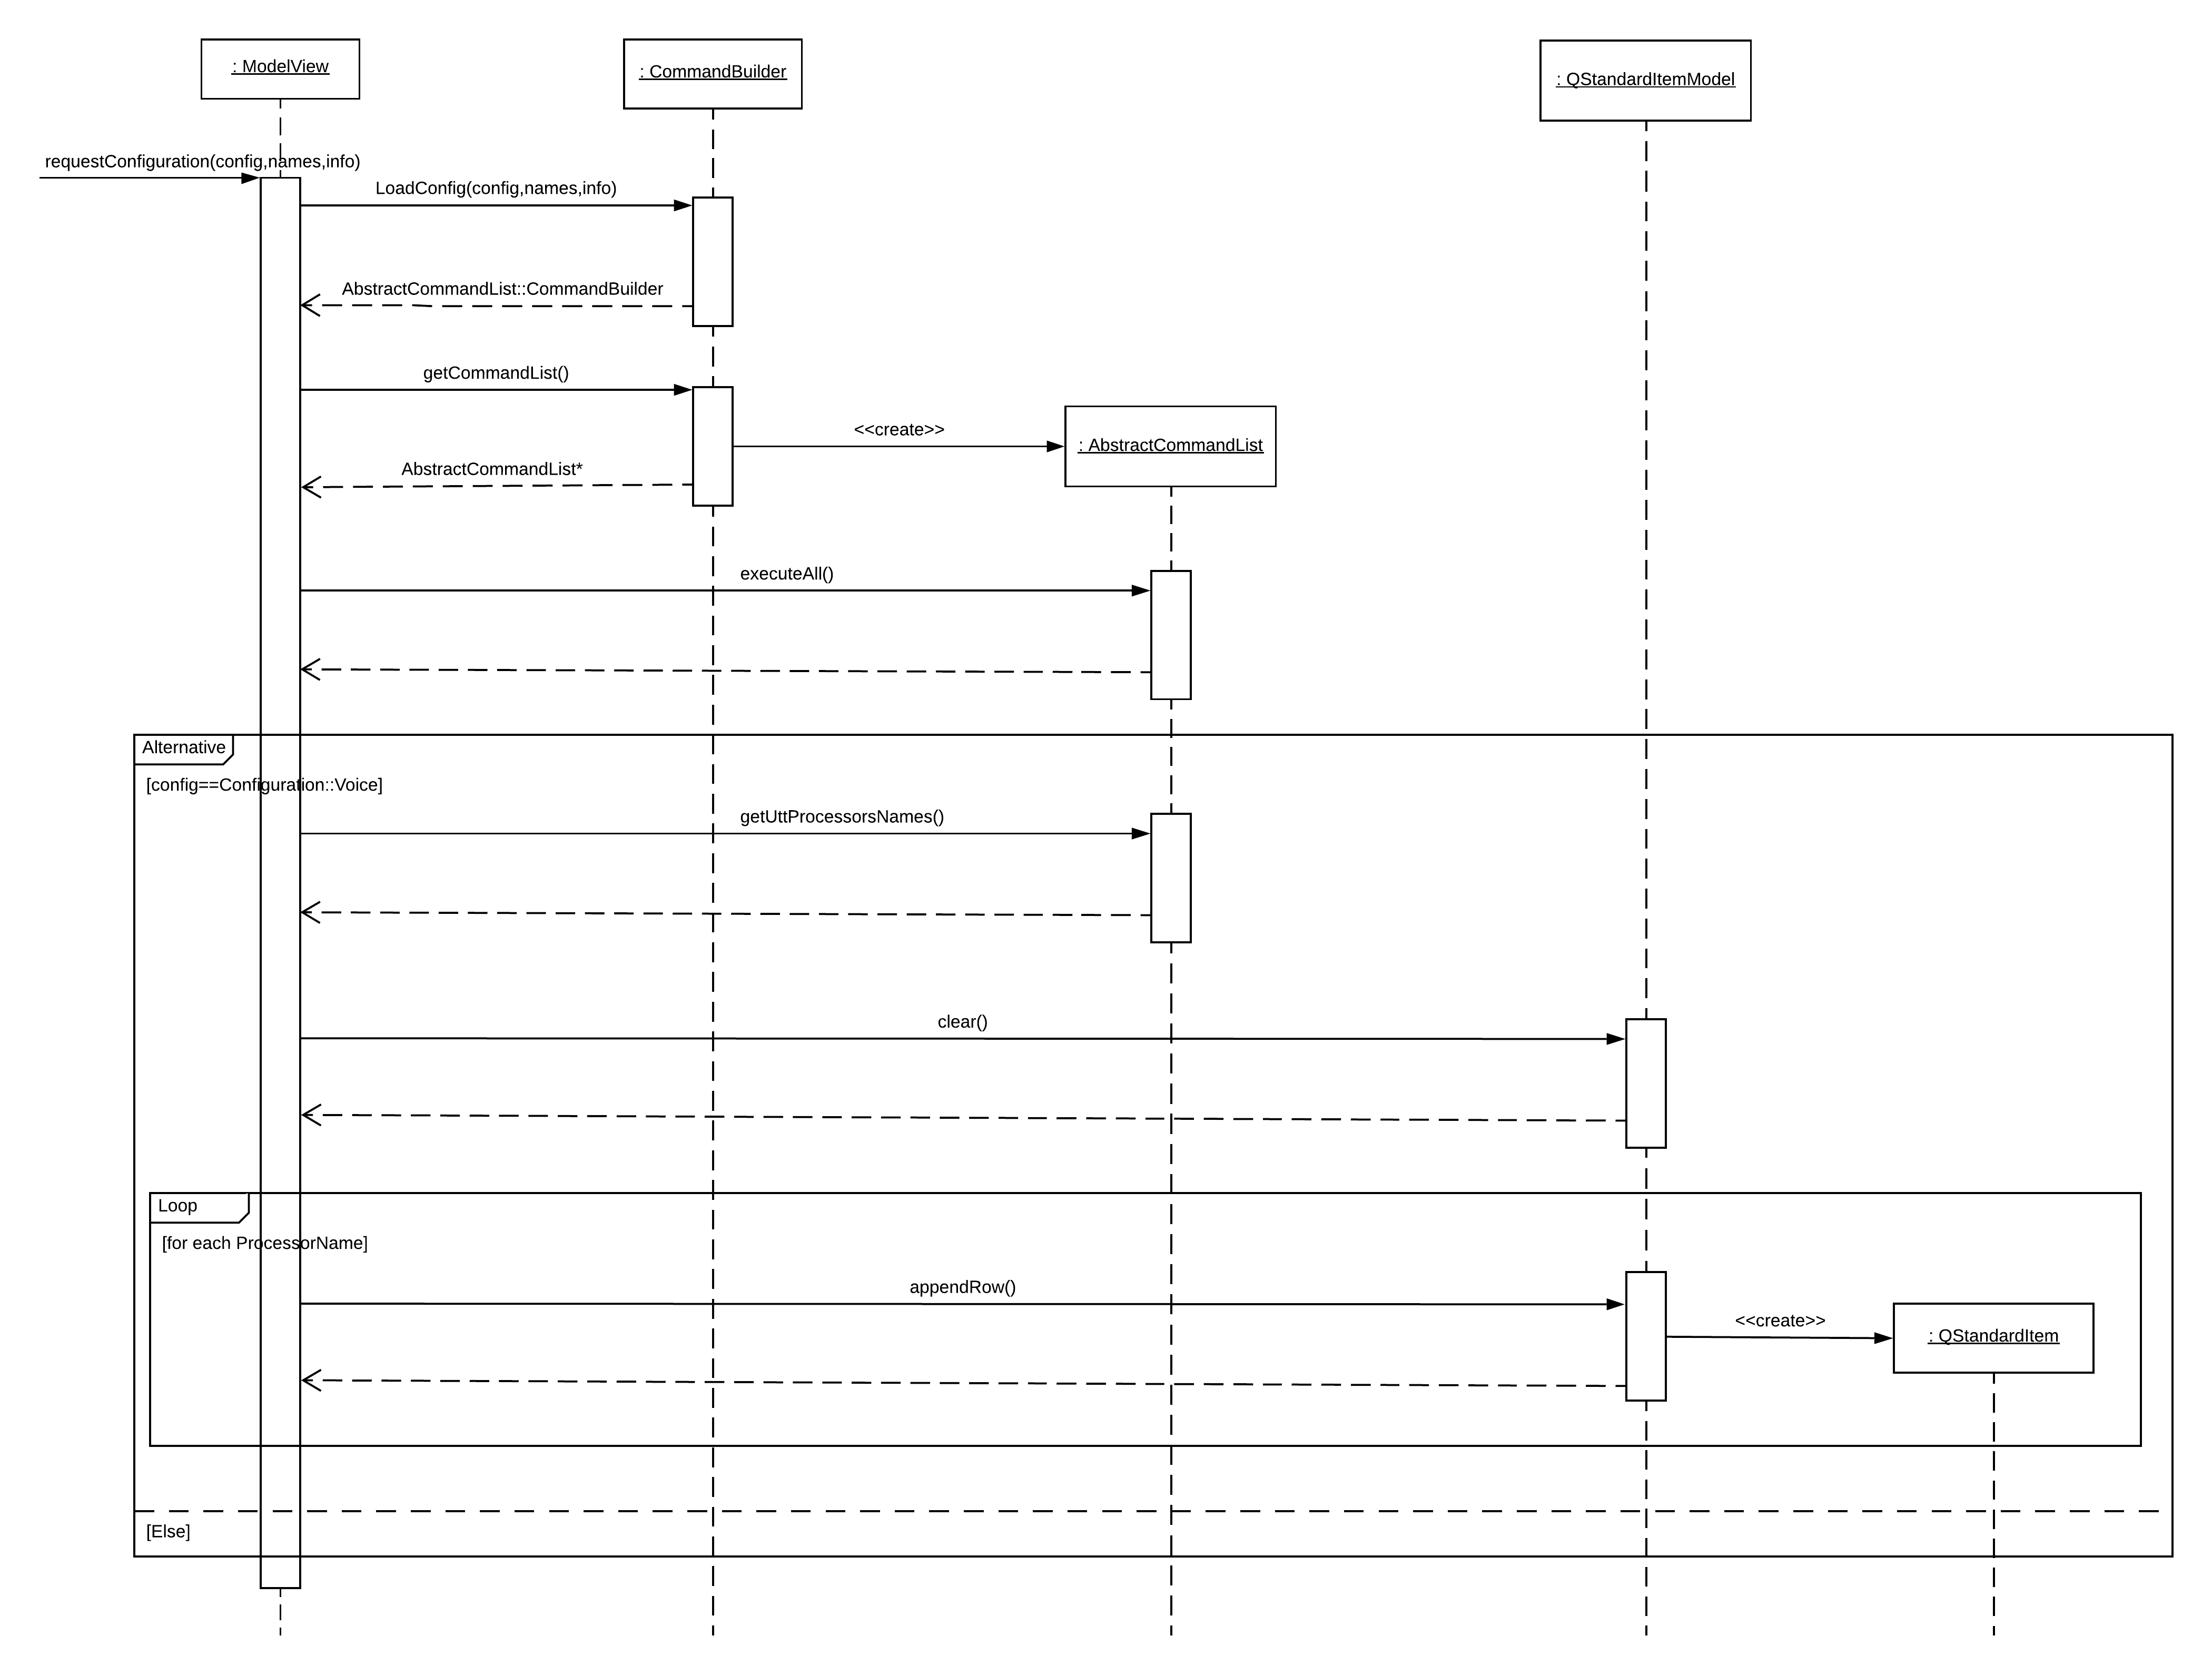
\includegraphics[scale=0.5]{CaricamentoVoice}
		\centering
		\caption{Diagramma di sequenza del processo di caricamento della voice}
	\end{figure}
	
	\subsection{Esecuzione utterance processor \\ selezionati}
	
	Il seguente diagramma di sequenza rappresenta il processo di esecuzione della lista di comandi selezionati dall'utente mediante l'interfaccia grafica.
	
	\begin{figure}[H]
		\hspace*{-30mm}
		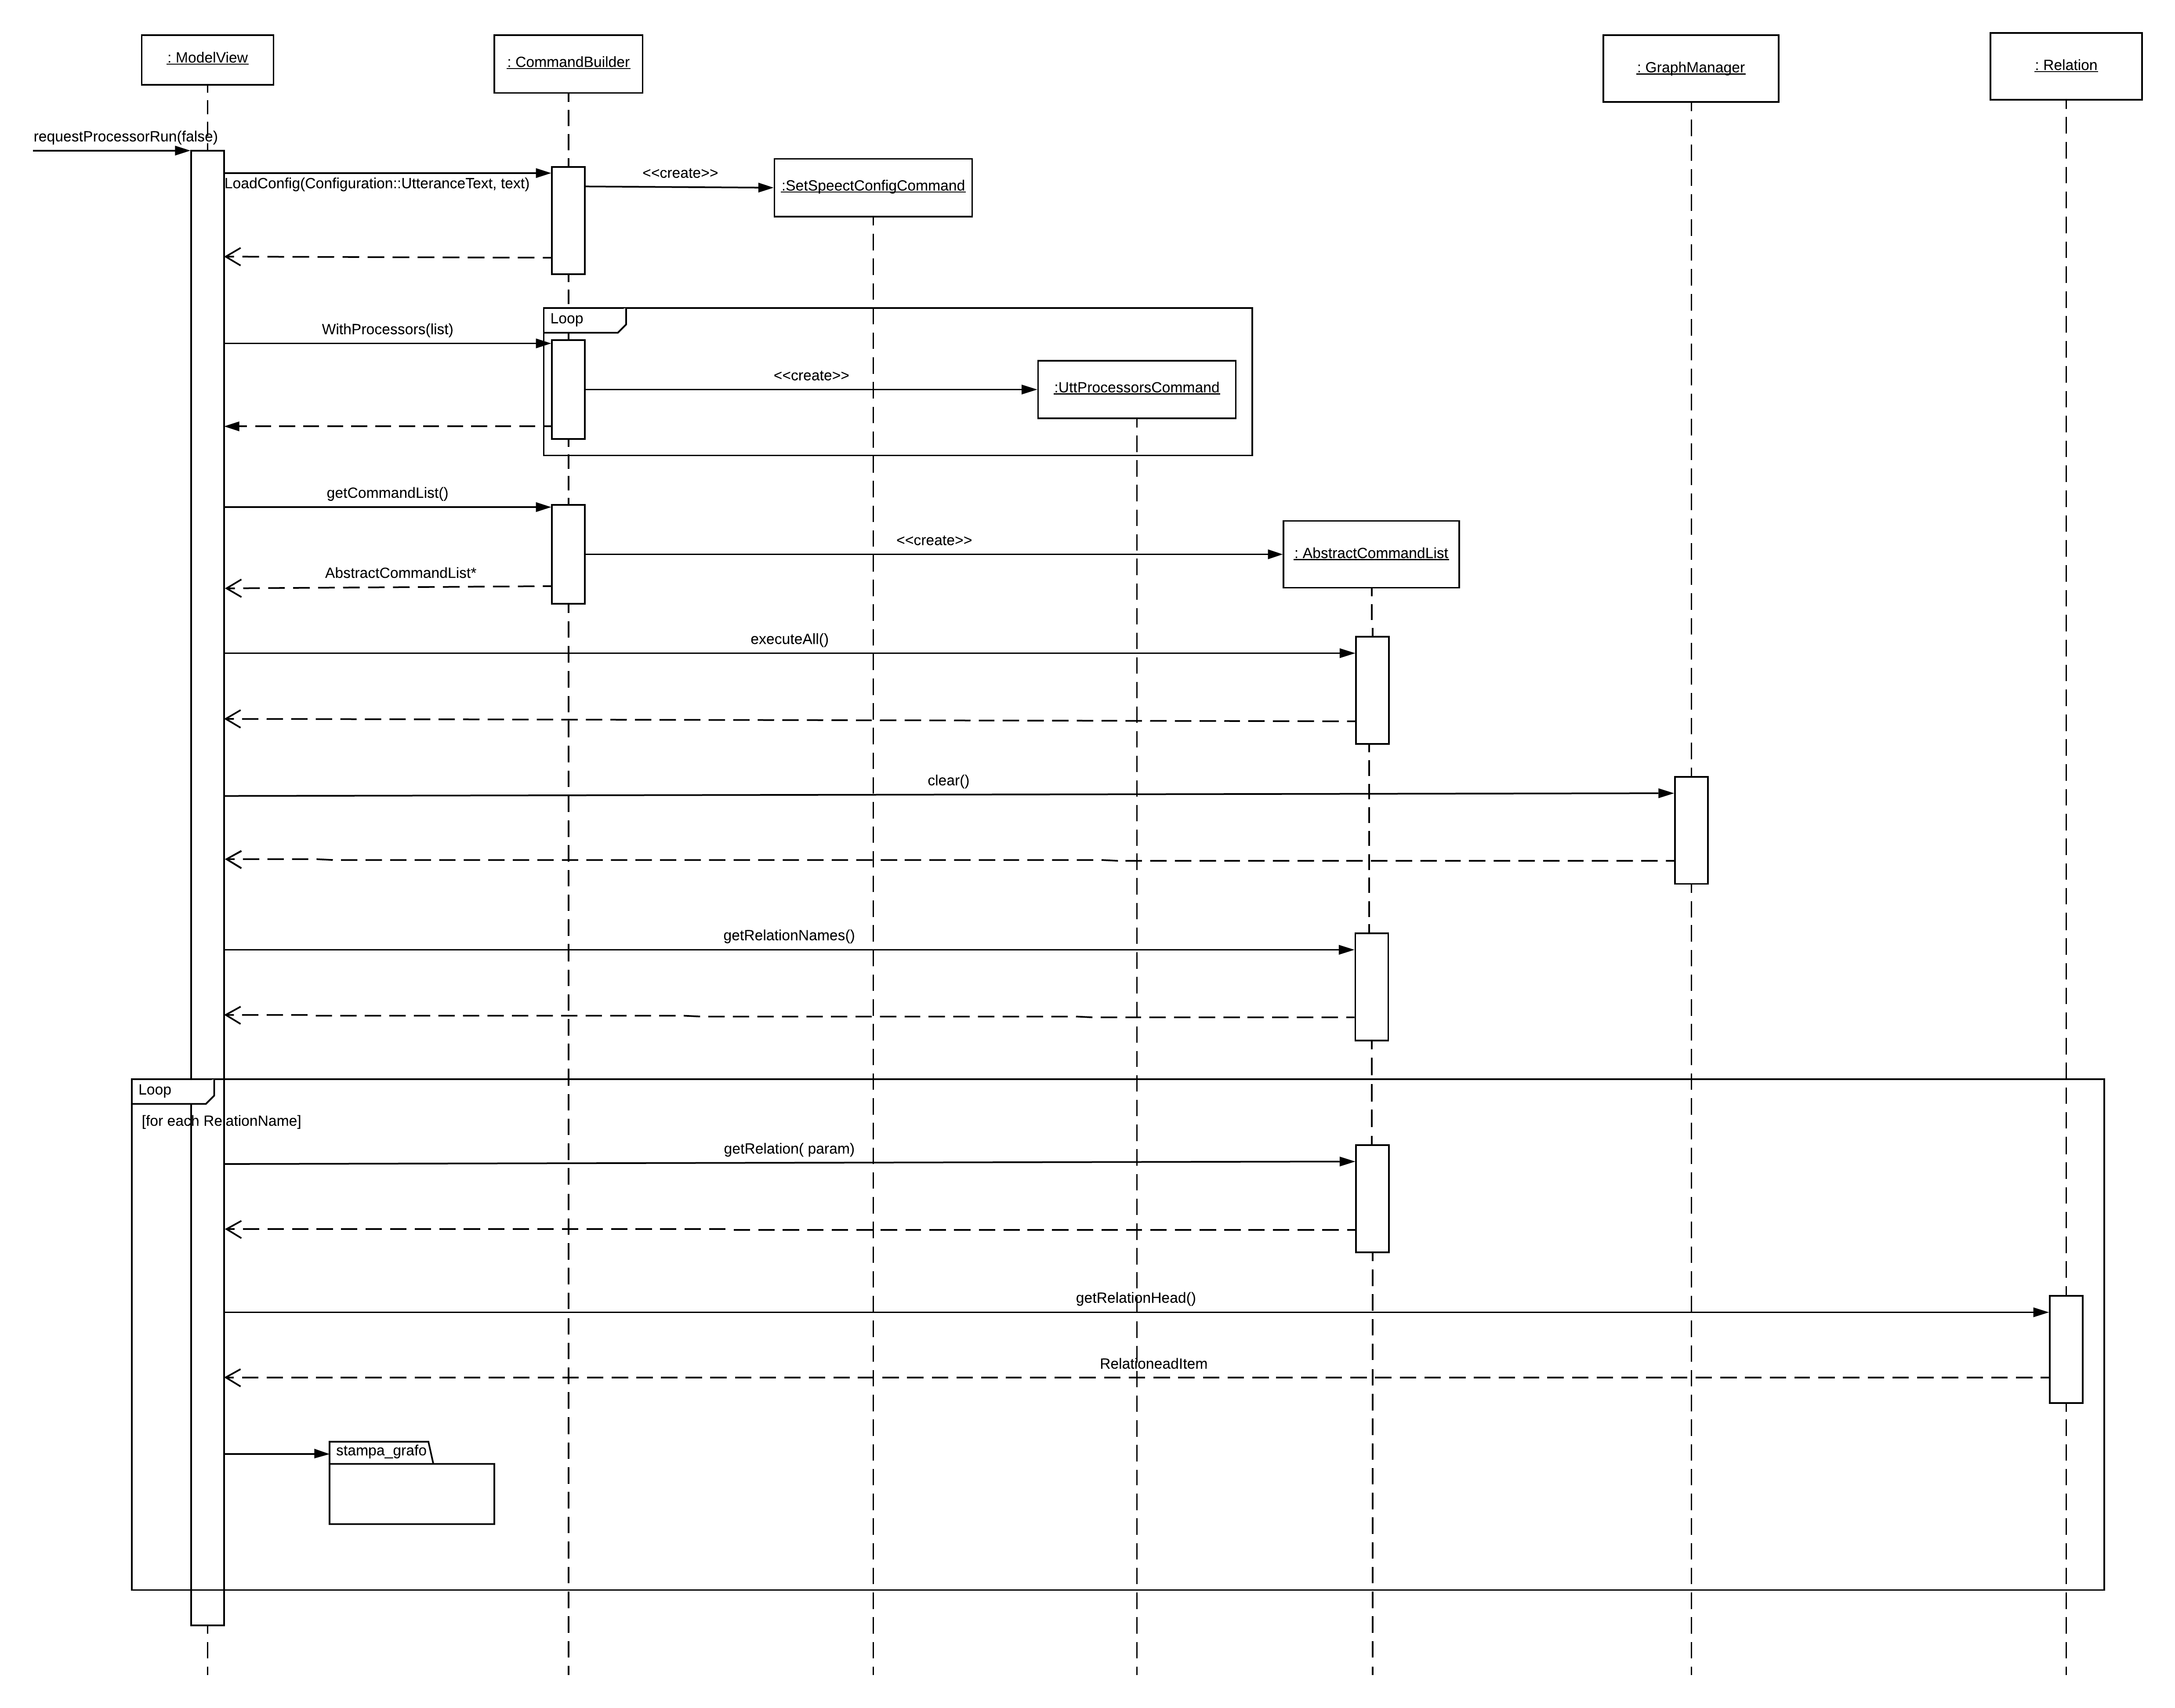
\includegraphics[scale=0.47]{EsecuzioneProcessor}
		\centering
		\caption{Diagramma di sequenza del processo di esecuzione degli utterance processor}
	\end{figure}

	\newpage
	
	\subsection{Stampa grafo}
	
	Il seguente diagramma di sequenza rappresenta il processo di stampa di un grafo.
	
	\begin{figure}[H]
		\hspace*{-25mm}
		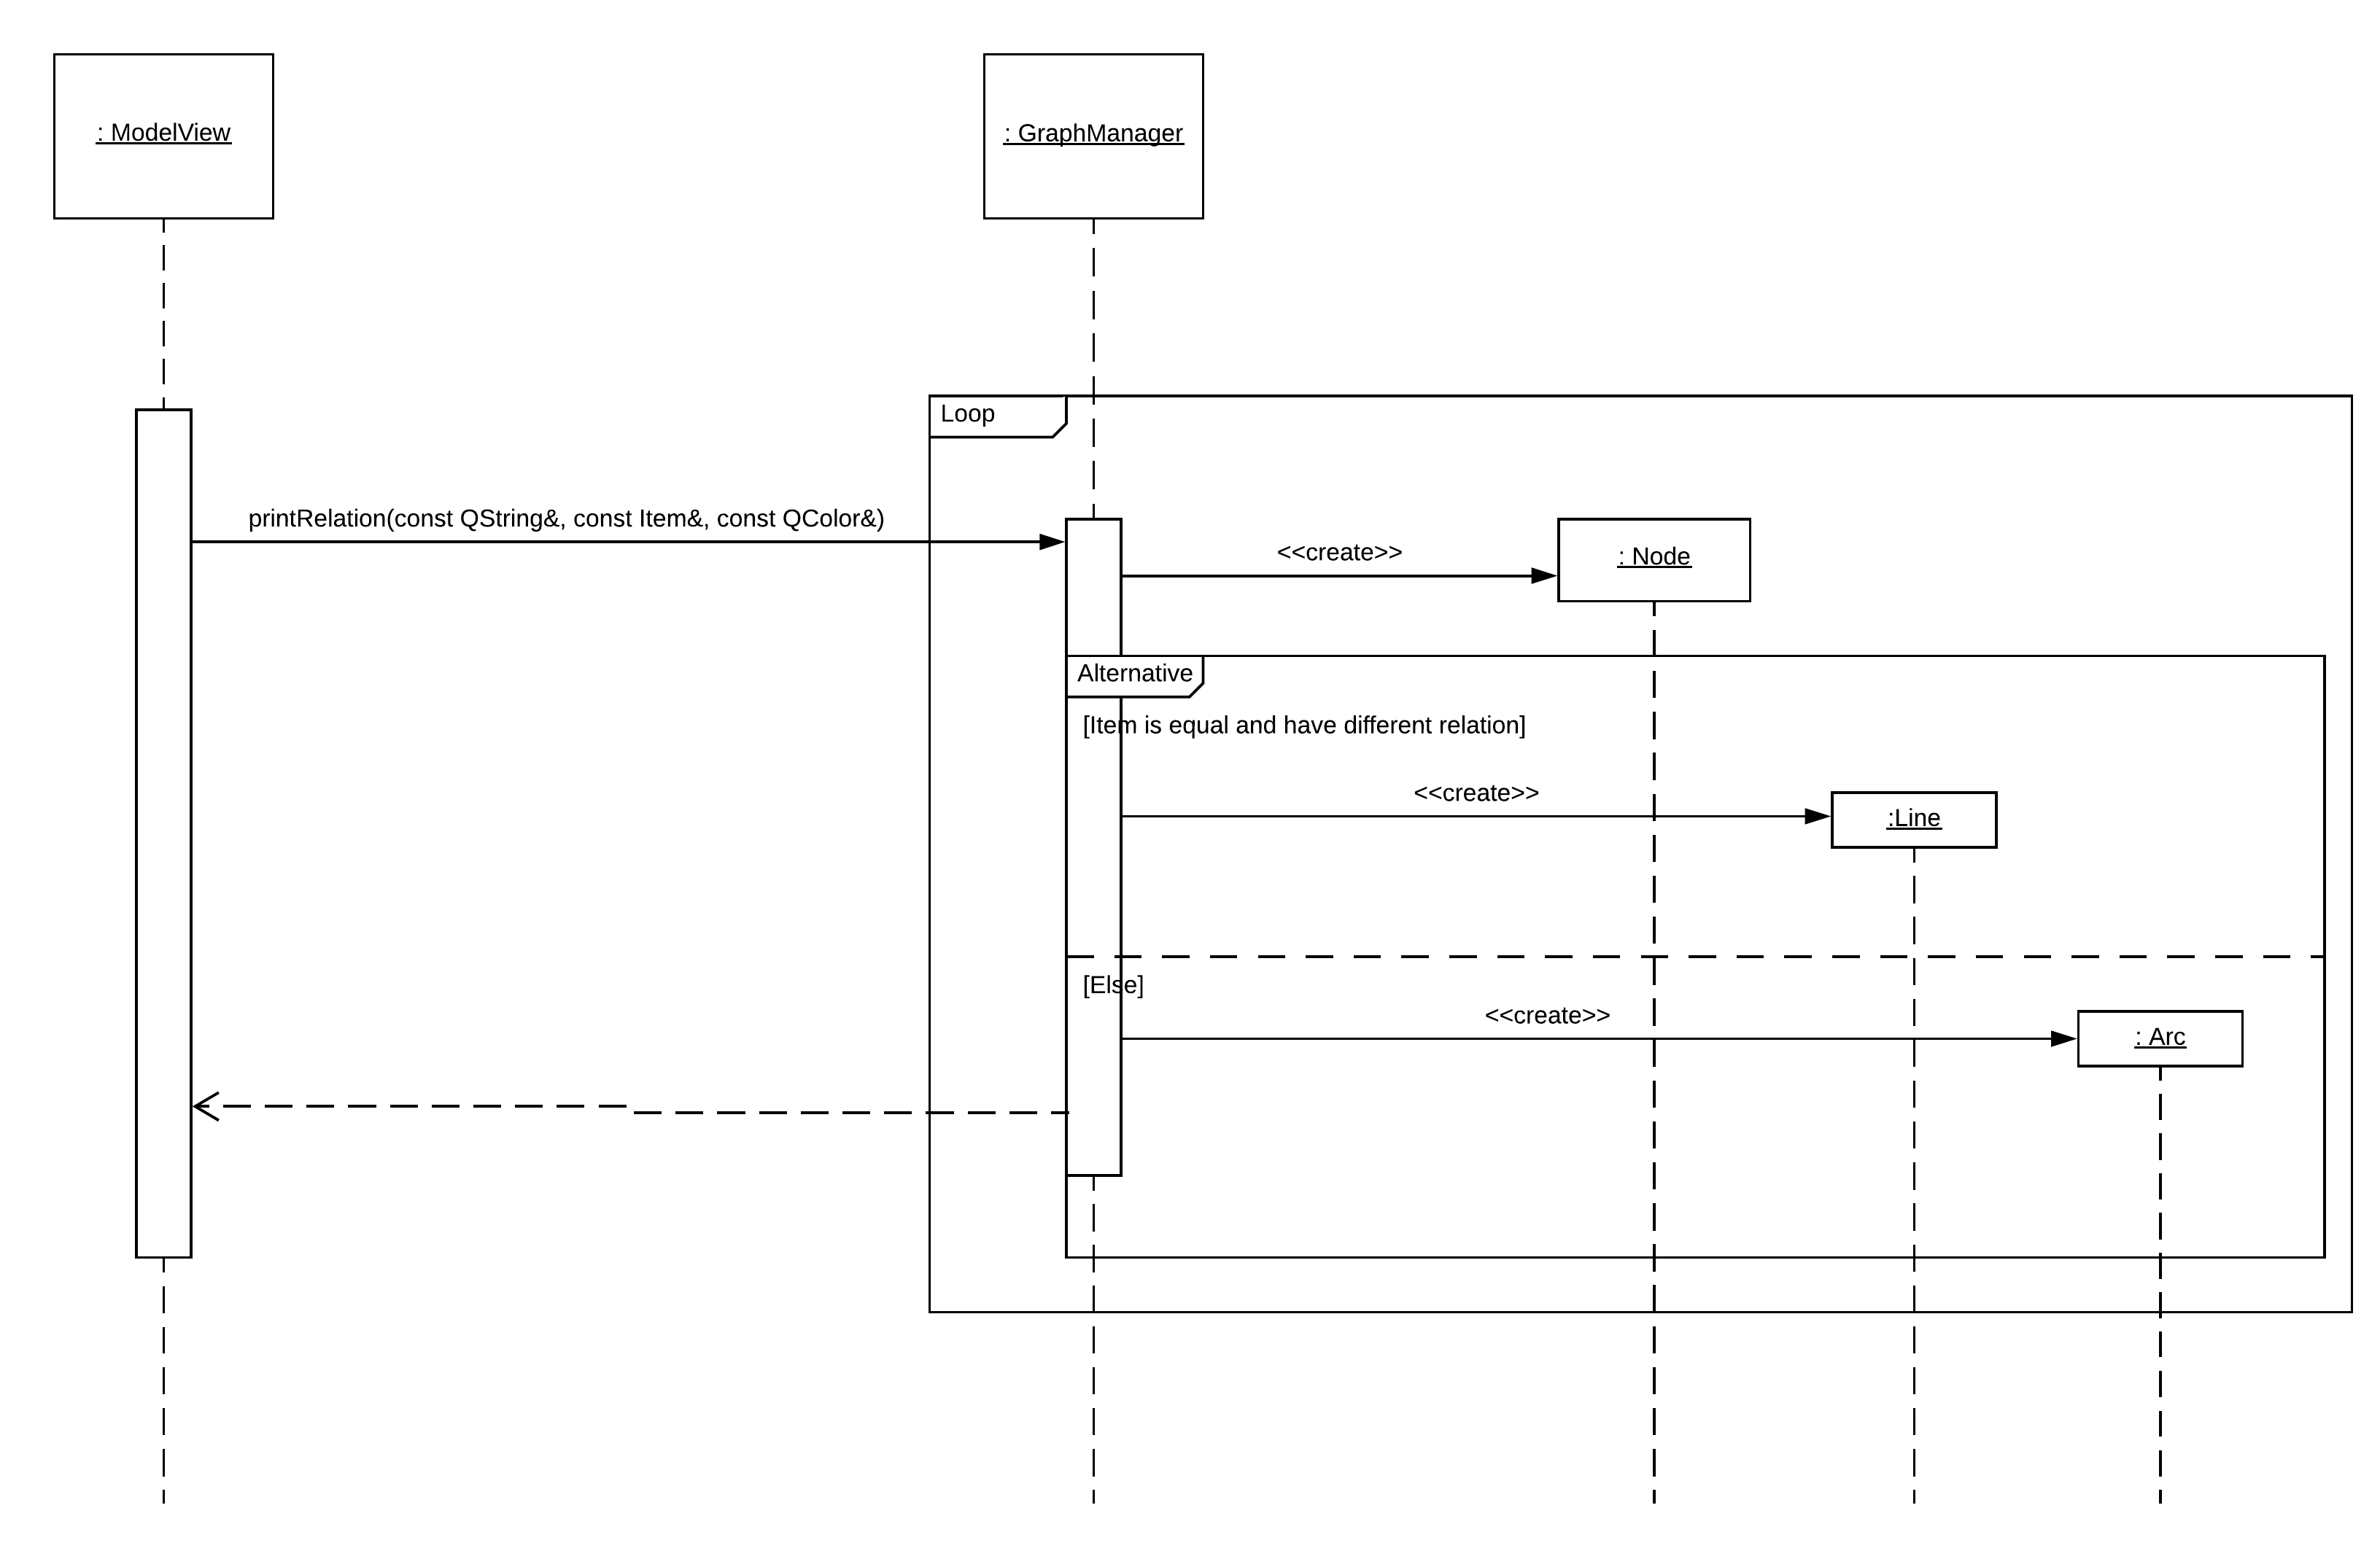
\includegraphics[scale=0.67]{StampaGrafo}
		\centering
		\caption{Diagramma di sequenza del processo di stampa del grafo}
	\end{figure}
	
	\chapter{Use case coperti}
	
	\section{Tabella della copertura degli use case}
	
	\begin{longtable}{|p{40mm}|p{40mm}|p{40mm}|}
		\hline
		\centering \textbf{Caso d'uso} & \textbf{Copertura architettura} &  \textbf{Copertura codice}\\
		
		\hline \centering UC1 & SODDISFATTO & SODDISFATTO \\
		\hline \centering UC2 & SODDISFATTO & SODDISFATTO\\
		\hline \centering UC3 & SODDISFATTO & SODDISFATTO\\
		\hline \centering UC3.1 & SODDISFATTO & SODDISFATTO\\
		\hline \centering UC4 & SODDISFATTO & \\
		\hline \centering UC4.1 & SODDISFATTO & \\
		\hline \centering UC5 & SODDISFATTO & SODDISFATTO\\
		\hline \centering UC6 &  &\\
		\hline \centering UC6.1 & SODDISFATTO & SODDISFATTO\\
		\hline \centering UC6.2 &  &\\
		\hline \centering UC6.3 &  &\\
		\hline \centering UC7 & SODDISFATTO & SODDISFATTO\\
		\hline \centering UC7.1 &  & \\
		\hline \centering UC7.2 & SODDISFATTO & SODDISFATTO\\
		\hline \centering UC7.3 & SODDISFATTO & SODDISFATTO\\
		\hline \centering UC8 &  & \\
		\hline \centering UC8.1 &  & \\
		\hline \centering UC9 &  & \\
		\hline \centering UC9.1 &  & \\
		\hline \centering UC10 & SODDISFATTO & \\
		\hline \centering UC10.1 &  & \\
		\hline \centering UC11 &  & \\
		\hline \centering UC11.1 &  & \\
		\hline \centering UC12 & SODDISFATTO & \\
		\hline \centering UC13 &  & \\
		\hline \centering \textbf{Caso d'uso} & \textbf{Copertura architettura} &  \textbf{Copertura codice}\\
		\hline \centering UC13.1 & SODDISFATTO & \\
		\hline \centering UC13.2 & SODDISFATTO & SODDISFATTO\\
		\hline \centering UC13.3 &  & \\
		\hline \centering UC13.4 &  & \\
		\hline \centering UC13.5 & SODDISFATTO & SODDISFATTO\\
		\hline
		
	\end{longtable}
	
	\newpage
	
	\section{Grafico della copertura degli use case}
		\begin{figure}[H]
		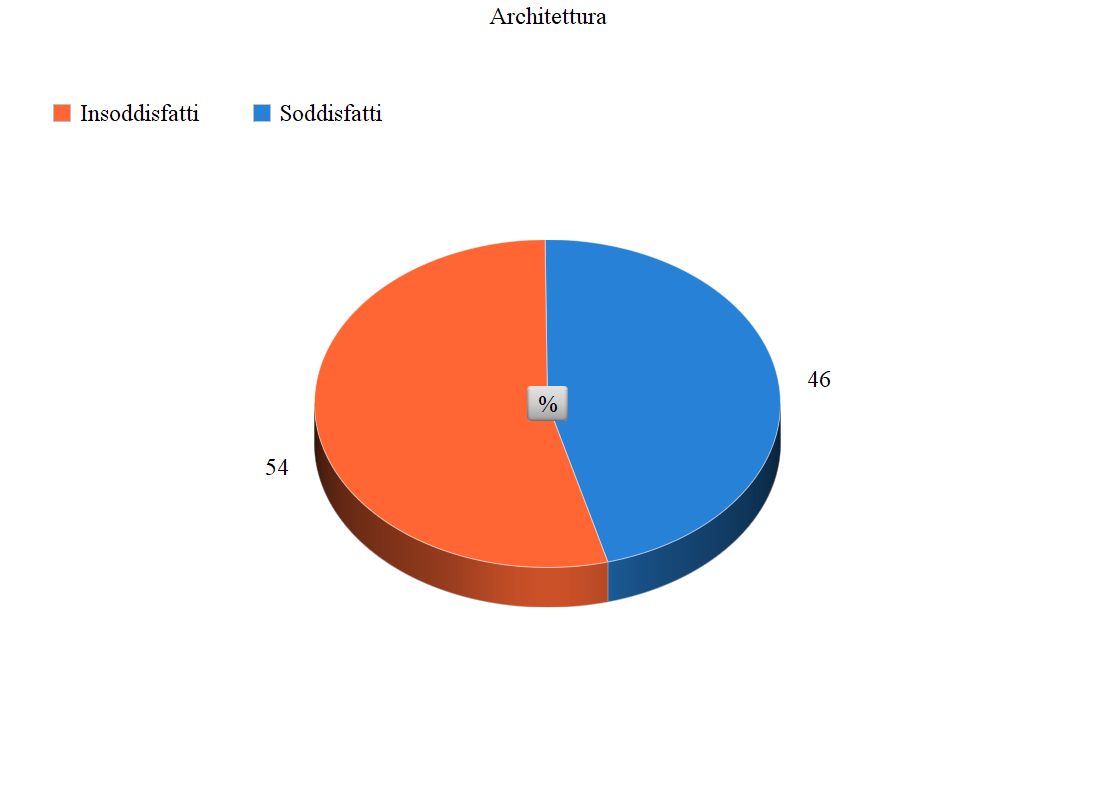
\includegraphics[scale=0.35]{casi_d'uso_Architettura}
		\centering
		\caption{Casi d’uso coperti nell'architettura}
	\end{figure}
	\begin{figure}[H]
		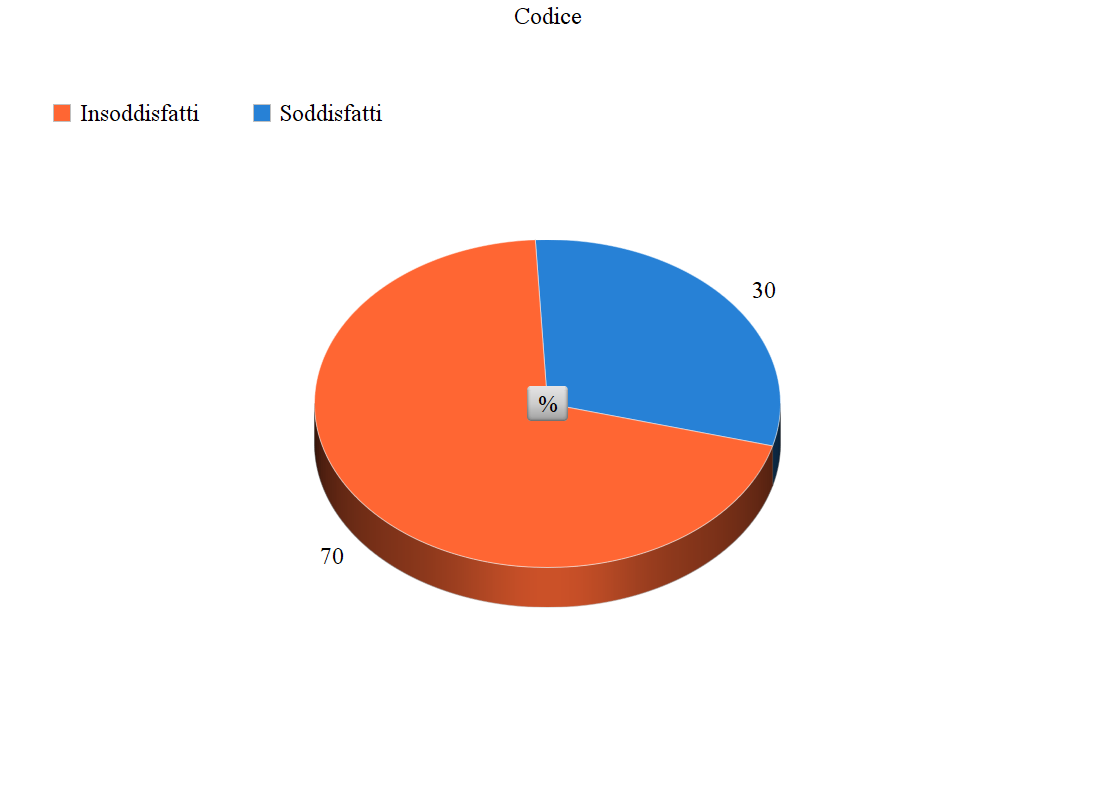
\includegraphics[scale=0.35]{casi_d'uso_codice}
		\centering
		\caption{Casi d’uso coperti nel codice}
	\end{figure}
	\chapter{Requisiti soddisfatti}
	
	\section{Tabella del soddisfacimento dei requisiti}
	\begin{longtable}{|p{40mm}|p{40mm}|p{40mm}|}
		\hline
		\centering \textbf{Requisito} & \textbf{Soddisfacimento architettura} &  \textbf{Soddisfacimento codice}\\
		
		\hline \centering ROF0 & SODDISFATTO & SODDISFATTO \\
		\hline \centering ROF1 & SODDISFATTO & SODDISFATTO\\
		\hline \centering ROF2 & SODDISFATTO & SODDISFATTO\\
		\hline \centering ROF2.1 & SODDISFATTO & SODDISFATTO\\
		\hline \centering ROF3 & SODDISFATTO & SODDISFATTO\\
		\hline \centering ROF3.1 & SODDISFATTO & \\
		\hline \centering ROF4 & SODDISFATTO &\\
		\hline \centering ROF4.1 & SODDISFATTO &\\
		\hline \centering ROF4.1.1 & SODDISFATTO &\\
		\hline \centering ROF4.2 & SODDISFATTO &\\
		\hline \centering ROF6 & SODDISFATTO &\\
		\hline \centering ROF7 & SODDISFATTO & SODDISFATTO\\
		\hline \centering ROF8 & SODDISFATTO & SODDISFATTO\\
		\hline \centering ROF8.1 & SODDISFATTO & \\
		\hline \centering ROF9 & SODDISFATTO & SODDISFATTO\\
		\hline \centering ROF9.1 & SODDISFATTO & \\
		\hline \centering ROF9.2 & SODDISFATTO & SODDISFATTO\\
		\hline \centering ROF9.3 & SODDISFATTO & SODDISFATTO\\
		\hline \centering ROF9.3.1 & SODDISFATTO & \\
		\hline \centering ROF9.5 & SODDISFATTO & SODDISFATTO\\
		\hline \centering ROF9.6 & SODDISFATTO & SODDISFATTO\\
		\hline \centering ROF9.7 & SODDISFATTO & SODDISFATTO\\
		\hline \centering ROF9.9 & SODDISFATTO & \\
		\hline \centering ROF14 & SODDISFATTO & SODDISFATTO\\
		\hline
		
	\end{longtable}
	\section{Grafico del soddisfacimento dei requisiti}
	\begin{figure}[H]
		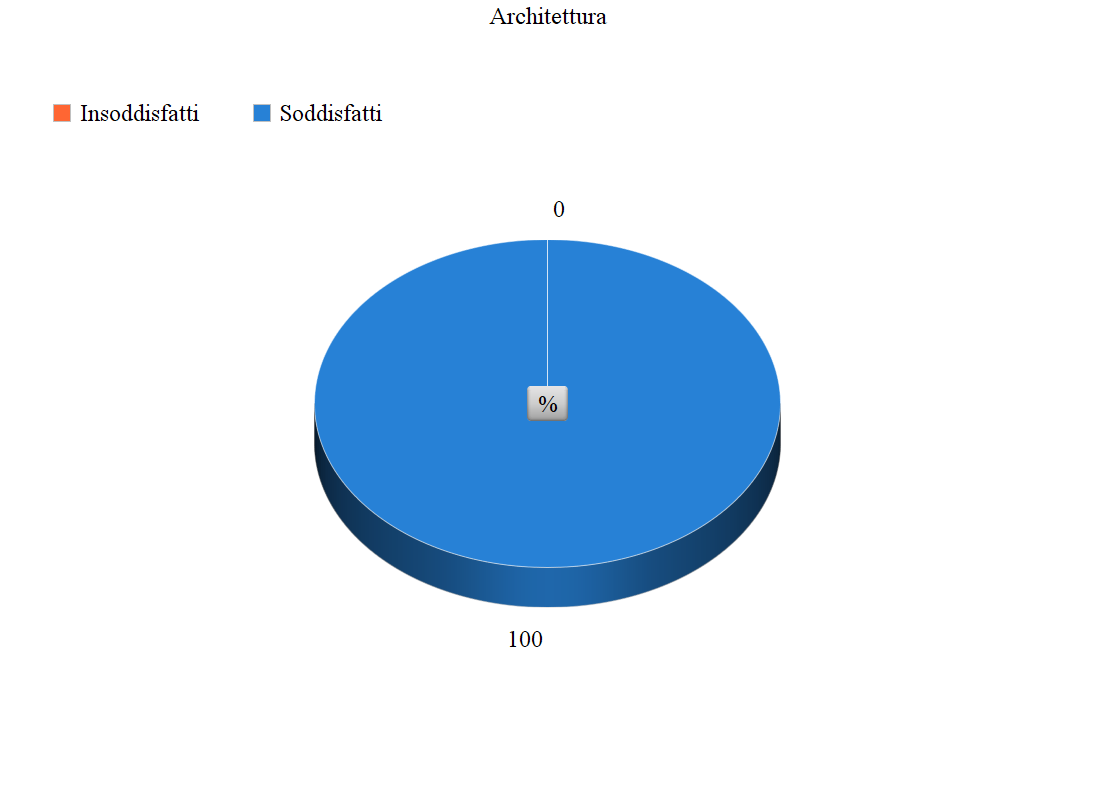
\includegraphics[scale=0.38]{Requisiti_obbligatori_architettura}
		\centering
		\caption{Requisiti obbligatori funzionali soddisfatti nell'architettura}
	\end{figure}
	\begin{figure}[H]
		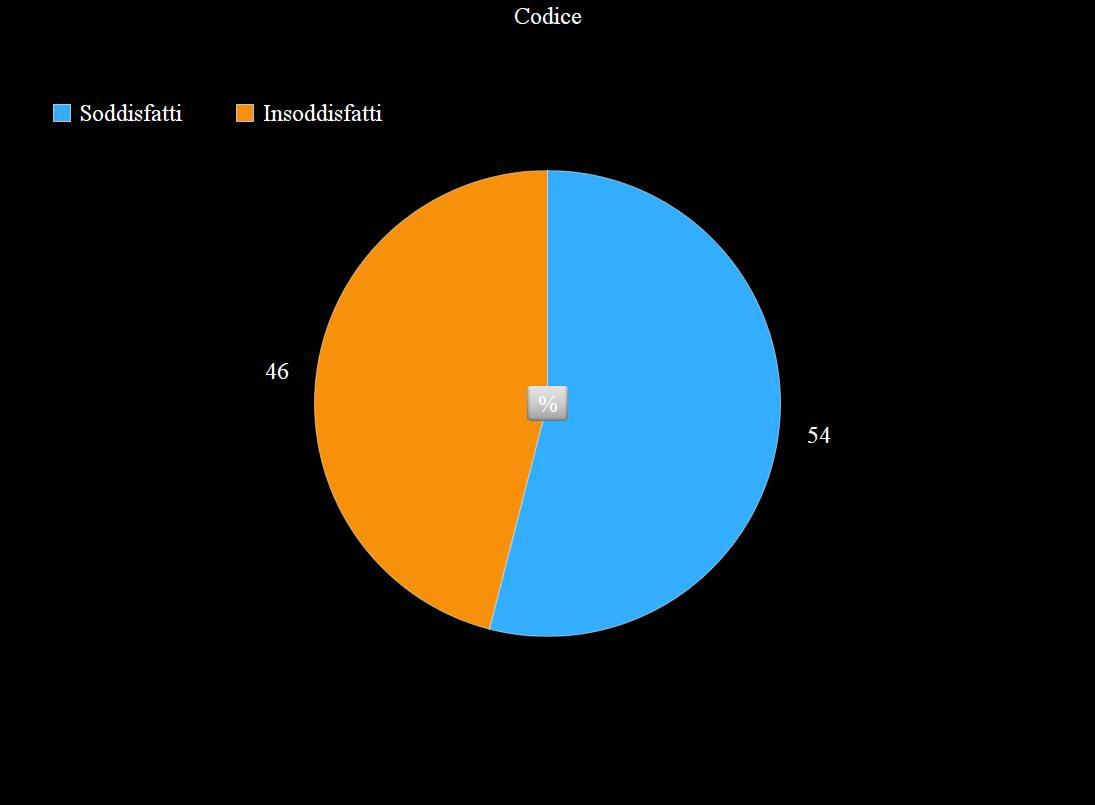
\includegraphics[scale=0.38]{Requisiti_obbligatori_codice}
		\centering
		\caption{Requisiti obbligatori funzionali soddisfatti nel codice}
	\end{figure}
	
	
	\chapter{Model-View-ViewModel}
	
	\section{Struttura del pattern}
	
	Il design pattern architetturale \textit{Model-View-ViewModel} (MVVM in breve) facilita la separazione dell'interfaccia grafica, che si tratti di linguaggio di markup o codice GUI, dallo sviluppo della logica di business o della logica di back-end, ovvero dal modello dei dati. Il \textit{ViewModel} di MVVM è un convertitore di valori, nel senso che è responsabile dell'esposizione (conversione) degli oggetti dati dal modello così da renderli facilmente gestibili e presentabili. Il pattern è riassunto dal seguente schema ed i suoi componenti principali sono di seguito approfonditi.\\
	
	\begin{figure}[H]
		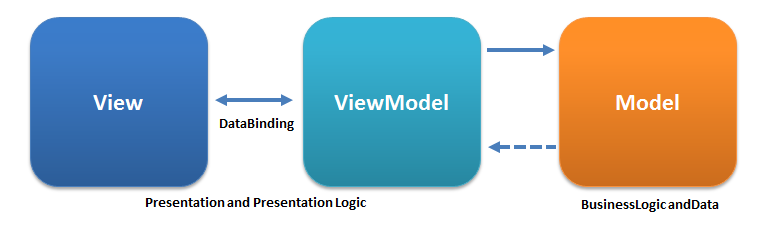
\includegraphics[scale=0.7]{MVVMPattern}
		\centering
		\caption{Diagramma generale dell'architettura MVVM}
	\end{figure}
	
	\noindent I tre componenti principali dell'architettura sono i seguenti:
	\begin{itemize}
		\item \textbf{Model}: il \textit{Model} (o modello) è un'implementazione del modello di dominio dell'applicazione ed include un modello dei dati affiancato alla logica di business e di validazione;
		\item \textbf{View}: la \textit{View} (o vista) è responsabile della definizione della struttura, del layout e dell'aspetto di ciò che l'utente visualizza su schermo. Idealmente, la vista è definita puramente con linguaggio di markup o generico codice GUI che non contiene la logica di business;
		\item \textbf{ViewModel}: la \textit{ViewModel} (o modello di presentazione) funge da intermediario tra la vista e il modello ed è responsabile della gestione della logica di visualizzazione. In genere, il ViewModel interagisce con il modello richiamandone i metodi delle classi: esso fornisce quindi dati dal modello in una forma facilmente utilizzabile dalla View. Il ViewModel recupera i dati dal modello, rendendoli disponibili alla View, e può riformattarli in un modo che renda più semplice la gestione della vista. Esso fornisce anche l'implementazione dei comandi che un utente dell'applicazione avvia nella vista (ad esempio, quando un utente clicca un pulsante nell'interfaccia grafica, tale azione può attivare un comando nel ViewModel) e può essere responsabile della definizione delle modifiche dello stato logico che influiscono su alcuni aspetti della visualizzazione della stessa, ad esempio l'indicazione che alcune operazioni sono in sospeso.
	\end{itemize}

	\section{Vantaggi offerti dal pattern}
	Il MVVM offre i seguenti vantaggi:
	
	\begin{itemize}
		\item Durante il processo di sviluppo, i programmatori e i designer possono lavorare in modo indipendente e simultaneamente sui loro componenti. Quest'ultimi possono concentrarsi sulla vista e, utilizzando appositi strumenti, generare facilmente dati di esempio con cui lavorare, mentre i programmatori possono lavorare sul modello di presentazione e sui componenti del modello;
		\item Gli sviluppatori possono creare test unitari per il ViewModel e per il Model senza utilizzare la View;
		\item È facile riprogettare l'interfaccia grafica dell'applicazione senza toccare il resto del codice, una nuova versione della vista dovrebbe poter funzionare con il modello di presentazione esistente;
		\item Se esiste un'implementazione del modello che incapsula la logica di business, potrebbe essere difficile o rischioso cambiarla. In questo scenario, il ViewModel funge da adattatore per le classi del Model e consente di evitare modifiche importanti al codice dello stesso.	
	\end{itemize}
	
\end{document}